
\documentclass[../_main/handlingar.tex]{subfiles}

\begin{document}
\motion{Namnbyte av funktionärspost}
Det är sannerligen dags för ett namnbyte av posten preferensmästare. Posten har tidigare kallats både mongomästare och mangomästare, och för en ung och fräsch kan det vara svårt att särskilja på alla dessa namn.

Oumph! är en nytt, trendigt, och fräscht köttsubstitut gjort på soja. Se bild. Observera att bilden visar ett serveringsförslag.

\begin{center}
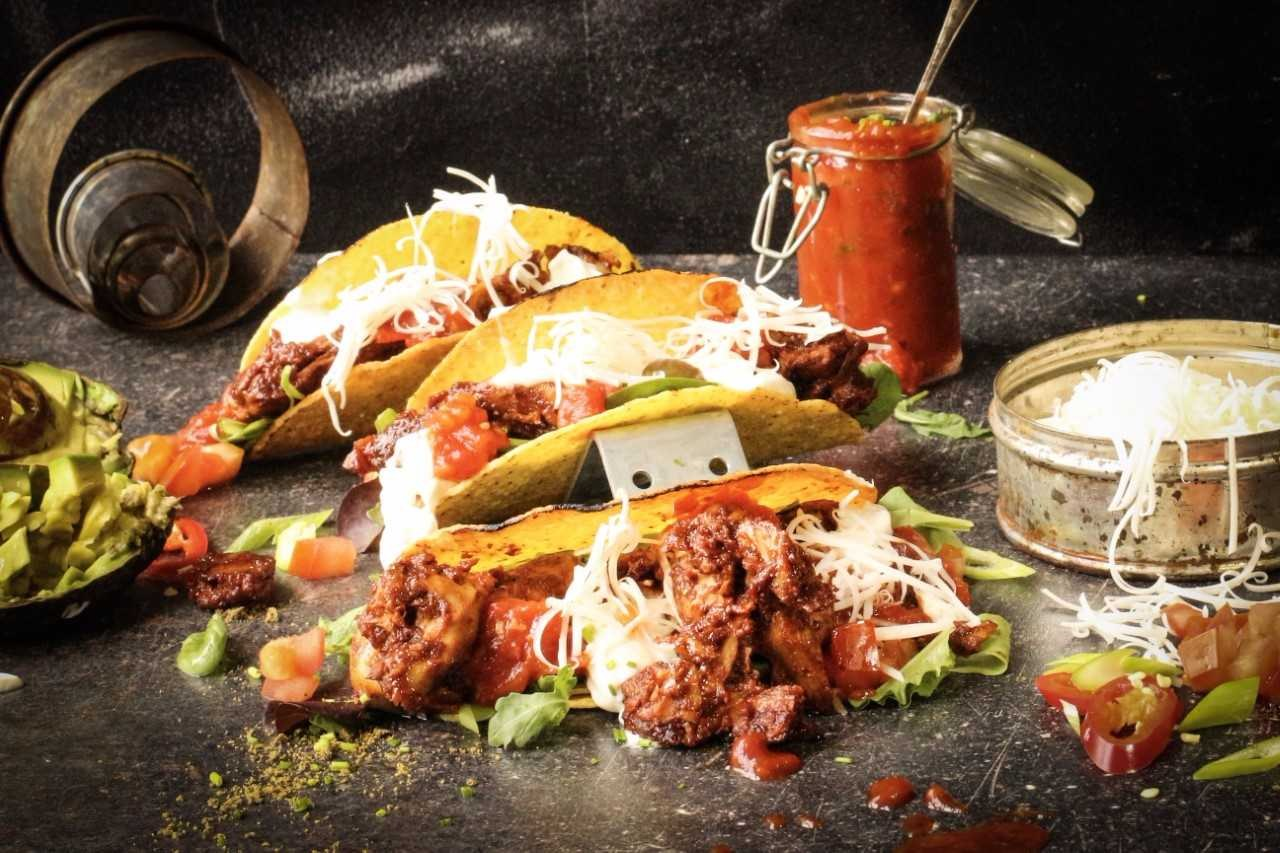
\includegraphics[height=8cm]{oumph.jpg}
\end{center}

Med detta i beaktelse yrkar motionären på

\begin{attsatser}
  \att funktionärsposten Preferensmästare byter namn till Oumph-meister, samt
  \att funktionärsposten Umph-meister byter namn till Disk-jockey (så kan E6 få hjälp efter sittningar).
\end{attsatser}

\begin{signatures}{1}
    Med vänliga hälsningar
    \signature{Johannes Koch}{E13}
\end{signatures}

\end{document}
